%%%%%%%%%%%%%%%%%%%%%
% Documento maestro %
%%%%%%%%%%%%%%%%%%%%%
\documentclass{fime}

%%%%%%%%%%%%%%%%%%%%%%%%%%%%%%%%%%%%%%%%%%%
% Cargando paquetes y definiendo opciones %
%%%%%%%%%%%%%%%%%%%%%%%%%%%%%%%%%%%%%%%%%%%
% Aquí puedes cargar los paquetes que vas a usar. La clase
% fime ya incluye babel, inputenc, graphicx y los de la AMS.
% Cargar un paquete está a tu libertad (y responsabilidad).
\usepackage{hyperref}
    \hypersetup{breaklinks=true,colorlinks=true,linkcolor=black,citecolor=black,urlcolor=black}

%%%%%%%%%%%%%%%%%%%%%
% Definiendo campos %
%%%%%%%%%%%%%%%%%%%%%
\def\titulo{Simulación de epidemias bajo medidas de contingencia}
\def\autor{Ericka Fabiola Vázquez Alcalá}
\def\matricula{1564189}
\def\grado{Maestría en Ciencias de la Ingeniería}
% En caso de que el grado tenga orientación o especialidad llenar el siguiente
% campo dejando un ESPACIO INICIAL, en caso contrario, dejar vacío
\def\orientacion{ con orientación en Sistemas}
% Coloca el mes con mayúscula inicial
\def\fecha{Agosto 2022}

\def\asesor{Dra. Satu Elisa Schaeffer}
\def\coasesor{Dr. José Arturo Berrones Santos}
\def\revisorA{ }
\def\revisorB{ }
% En el caso de que tu tesis sea de doctorado activa la variable cambiándola a \doctoradotrue
% y define tus otros dos revisores
\newif\ifdoctorado\doctoradofalse
\def\revisorC{}
\def\revisorD{}
% El visto bueno siempre va
\def\vobo{Dr. Simón Martínez Martínez}

%%%%%%%%%%%%%%%%%%%%%%%
% Inicia el documento %
%%%%%%%%%%%%%%%%%%%%%%%
\begin{document}

\frontmatter
\pagestyle{main}

%%%%%%%%%%%%%%%%%%%%%%%%
% Primer portada: UANL %
%%%%%%%%%%%%%%%%%%%%%%%%
\thispagestyle{empty}

\begin{scshape}
\begin{center}
	{\Large \uanl} \\[5mm]
	{\large \fime} \\[5mm]
	{\large \depg}
	\vskip15mm
	
\includegraphics[height=55mm]{uanl}
	\vskip12mm
	\begin{tabular}{p{11cm}}
		\centering
		{\large \titulo}
	\end{tabular}
	\vskip7mm
	{por}\\[7mm]
	{\large \autor}\\[7mm]
        % Si en tu posgrado la tesis no es opcional (como sí lo es en licenciatura), no modifiques esta línea:
	{como requisito parcial para obtener el grado de}\\[3mm]
	\MakeUppercase{\grado}\\
	\orientacion
	\vfill
	\fecha
\end{center}
\end{scshape}

%%%%%%%%%%%%%%%%%%%%%%%%%
% Segunda portada: FIME %
%%%%%%%%%%%%%%%%%%%%%%%%%
\newpage
\thispagestyle{empty}

\begin{scshape}
\begin{center}
	{\Large\uanl} \\[5mm]
	{\large\fime} \\[5mm]
	{\large\depg}
	\vskip16mm
	
\includegraphics[height=50mm]{fime}
	\vskip16mm
	\begin{tabular}{p{11cm}}
		\centering
		{\large \titulo}
	\end{tabular}
	\vskip7mm
	{por}\\[7mm]
	{\large \autor}\\[7mm]
        % Si en tu posgrado la tesis no es opcional (como sí lo es en licenciatura), no modifiques esta línea:
	{como requisito parcial para obtener el grado de}\\[3mm]
	\MakeUppercase{\grado}\\
	\orientacion
	\vfill
	\fecha
\end{center}
\end{scshape}

%%%%%%%%%%%%%%%%%%%%%%%%%%%%%
% Carta del comité de tesis %
%%%%%%%%%%%%%%%%%%%%%%%%%%%%%
\newpage
\thispagestyle{empty}
\enlargethispage{5mm}

{\renewcommand{\baselinestretch}{1.1}\selectfont
\begin{center}\vspace*{-25mm}\hspace*{-10mm}
\begin{minipage}{170.5mm}
\hspace{-1.5mm}
\includegraphics[height=20mm]{uanl}\hfill\raise1mm\hbox{
\includegraphics[height=18.5mm]{fime}}
\hrule\vspace{0.5mm}
\scalebox{.5}{\MakeUppercase{\uanl}}\hfill\scalebox{.5}{\MakeUppercase{\fime}}\medskip
\end{minipage}
\vskip4mm{\sc\large\uanl\\\fime\\[3pt]\depg}\vskip6mm
\end{center}

Los miembros del Comité de Tesis recomendamos que la Tesis  {\it\titulo}, realizada por el alumno \autor, con número de matrícula \matricula, sea aceptada para su defensa como requisito parcial para obtener el grado de \grado\orientacion.
\ifdoctorado\vskip10mm\else\vskip8mm\fi

\begin{center}
El Comité de Tesis\\
\ifdoctorado\vskip15mm\else\vskip25mm\fi

\ifdoctorado{%%%
\begin{tabular}{p{37mm}p{21mm}p{12mm}p{21mm}p{37mm}}
	\cline{1-2} \cline{4-5}
	\multicolumn{2}{c}{\asesor} & & \multicolumn{2}{c}{\coasesor} \\
	\multicolumn{2}{c}{Asesor}   & & \multicolumn{2}{c}{Coasesor}   \\[17mm]
	\cline{1-2} \cline{4-5}
	\multicolumn{2}{c}{\revisorA} & & \multicolumn{2}{c}{\revisorB} \\
	\multicolumn{2}{c}{Revisor}   & & \multicolumn{2}{c}{Revisor}   \\[17mm]
	\cline{1-2} \cline{4-5}
	\multicolumn{2}{c}{\revisorC} & & \multicolumn{2}{c}{\revisorD} \\
	\multicolumn{2}{c}{Revisor}   & & \multicolumn{2}{c}{Revisor}   \\[2mm]
	& \multicolumn{3}{c}{Vo. Bo.} & \\[14mm]
	\cline{2-4}
	& \multicolumn{3}{c}{\vobo}   & \\
	& \multicolumn{3}{c}{Subdirector de Estudios de Posgrado}   & \\ &&&&
\end{tabular}
}\else{%%%
\begin{tabular}{p{37mm}p{21mm}p{12mm}p{21mm}p{37mm}}
	\cline{1-2} \cline{4-5}
	\multicolumn{2}{c}{\asesor} & & \multicolumn{2}{c}{\coasesor} \\
	\multicolumn{2}{c}{Asesor}   & & \multicolumn{2}{c}{Coasesor}   \\[17mm]
	\cline{1-2} \cline{4-5}
	\multicolumn{2}{c}{\revisorA} & & \multicolumn{2}{c}{\revisorB} \\
	\multicolumn{2}{c}{Revisor}   & & \multicolumn{2}{c}{Revisor}   \\[2mm]
	& \multicolumn{3}{c}{Vo. Bo.} & \\[17mm]
	\cline{2-4}
	& \multicolumn{3}{c}{\vobo}   & \\
	& \multicolumn{3}{c}{Subdirector de Estudios de Posgrado}   & \\ &&&&
\end{tabular}
}\fi%%%

\vfill

\snnl, \MakeLowercase{\fecha}

\end{center}}

% Dedicatoria

\thispagestyle{empty}
\vspace*{17mm}

\begin{flushright}
\begin{itshape}

A mi papá en el cielo, a mi mamá, y a Gerardo.

\end{itshape}
\end{flushright}



\tableofcontents
\listoffigures
\listoftables

%Agradecimientos

\chapter{Agradecimientos}
\markboth{Agradecimientos}{}

Mis más profundos agradecimientos a la Universidad Autónoma de Nuevo León (UANL) por la oportunidad que me ha brindado de formarme en sus aulas desde el nivel medio superior, y por los apoyos económicos derivados de los proyectos \textit{Simulación de epidemias bajo medidas de contingencia} (CE1842-21, Mayo 2021 - Diciembre 2021) y \textit{Exploración algorítmica de relaciones entre calidad de aire y bienestar} (CE1421-20, Agosto 2020 - Diciembre 2020). A la Facultad de Ingeniería Mecánica y Eléctrica, por acogerme para mis estudios de maestría. Al Consejo Nacional de Ciencia y Tecnología por el financiamiento otorgado para que pudiera estudiar de tiempo completo.

Agradezco al Posgrado en Ingeniería de Sistemas por recibirme como estudiante de maestría, en especial a mis asesores Elisa Schaeffer y José Arturo Berrones Santos, sin cuya orientación y apoyo no habría podido obtener este grado. También a mis revisores por aceptar formar parte de mi comité de tesis y por sus valiosas observaciones.
%Resumen

\chapter{Resumen}
\markboth{Resumen}{}

{\renewcommand{\baselinestretch}{1.1}\selectfont
{\setlength{\leftskip}{10mm}
\setlength{\parindent}{-10mm}

\autor.

Candidato para obtener el grado de \grado\orientacion.

\uanl.

\fime.

Título del estudio: \textsc{\titulo}.

\noindent Número de páginas: \pageref*{lastpage}.}

%%% Comienza a llenar aquí
\paragraph{Objetivos y método de estudio:}
Aquí debes poner tus objetivos y métodos de estudio. (Este es el formato).

\paragraph{Contribuciones y conlusiones:}
Y aquí tus contribuciones y conclusiones. (También es parte del formato).

\bigskip\noindent\begin{tabular}{lc}
\vspace*{-2mm}\hspace*{-2mm}Firma del asesor: & \\
\cline{2-2} & \hspace*{1em}\asesor\hspace*{1em}
\end{tabular}}



\mainmatter
\pagestyle{fime}

%%% Haz un documento para cada capítulo
\chapter{Introducción}

La humanidad ha sido asediada por enfermedades infecciosas a lo largo de la historia. Ejemplos en la era moderna incluyen las epidemias del SARS, MERS, influenza AH1N1 ébola y en la actualidad, el SARS CoV-2, virus que causa la enfermedad conocida como \textit{covid-19}. Ante estas eventualidades, gobiernos de distintos niveles deben adoptar medidas prontas y efectivas para evitar una crisis de salud pública. Sin embargo es difícil saber el impacto que tendrán las acciones tomadas ante un sistema complejo y dinámico, como lo es la propagación de una enfermedad en una población. Ante la inviabilidad logística, y quizá ética, de ensayar distintas medidas directamente a nivel población, surge la necesidad de realizar ensayos computacionales mediante modelos matemáticos de la enfermedad. La naturaleza aleatoria y evolutiva de los procesos de contagio hace de las simulaciones estocásticas una de las maneras más efectivas de estudiar y predecir el fenómeno.

Las técnicas de simulación multi-agente permiten analizar y cuantificar los efectos de distintas medidas de contención ante la propagación de enfermedades, tales como el distanciamiento social, el uso de cubrebocas,  o el aislamiento social, además de interacciones con otros factores como la densidad poblacional, nivel socioeconómico y la calidad del aire. La comprensión de estas diferencias conlleva a una toma de decisiones facilitada y basada en evidencia científica. Aunado a esto, representar las conexiones e interacciones entre nuestros agentes por medio de una red, permite el uso de técnicas matemáticas bien estudiadas de teoría de grafos y sistemas de propagación en redes. Combinando estas dos metodologías, confiamos que las redes complejas multi-agentes son idóneas para la simulación estocástica de epidemias bajo medidas de contención.

\section{Hipótesis y objetivo}
La hipótesis es que la simulación de modelos epidemiológicos por medio de redes multi-agente permite observar y cuantificar el impacto que distintas medidas de contención tienen en la propagación de una enfermedad infecciosa. Esto permitiría una toma de decisiones públicas más informada y con mejores resultados.

El objetivo general es diseñar, implementar y analizar una simulación multi-agente epidemiológica en una red que permita medir los efectos que tienen distintas medidas de contención contra el contagio y propagación de una enfermedad infecciosa. Los objetivos específicos para el presente trabajo son:
\begin{description}
\item[Modelación.] Diseñar una simulación multi-agente en red de un modelo epidemiológico, el cuál permita medir la propagación de una enfermedad infecciosa bajo distintas medidas de contingencia. Específicamente, del uso de cubrebocas, distanciamiento social y aislamiento.

\item[Implementación.] Implementar un prototipo computacional del modelo desarrollado para explorar la magnitud del impacto que distintas medidas de contingencia, o la ausencia de estas, tengan en medidas clave de la propagación de la enfermedad, como lo son porcentaje final de infectados, duración de la epidemia, máxima cantidad de infectados simultáneamente.

\item[Visualización.] Crear visualizaciones de la propagación de la enfermedad en una red acorde a los resultados obtenidos con la implementación del modelo mencionado, así como del impacto de las medidas de contingencia. 
\end{description}


\section{Estructura de la tesis}

En el capítulo \ref{ch:background} se describen los conceptos clave necesarios para la comprensión de este trabajo. En el capítulo \ref{ch:litreview} se realiza una revisión de la literatura relacionada al tema. En el capítulo \ref{ch:method} se describe la metodología empleada para la solución del problema. Por último en el capítulo \ref{ch:results} se muestran los resultados obtenidos de las experimentaciones y en el capítulo \ref{ch:conclusions} se describen las conclusiones obtenidas.


\chapter{Marco teórico}\label{ch:background}

Un grafo (o red) simple es una dupla $G = (V, E)$ que consiste de un conjunto de vértices $V$ y un conjunto de aristas $E = \{ \{u, v\} : u, v \in E, u \neq v\}$. Un sistema basado en agentes consiste de un conjunto de entidades heterogéneas, llamadas agentes, que interactúan entre sí acorde a un sistema de reglas. A través de estas interacciones emergen fenómenos a nivel del sistema. Una red o grafo multi-agente es una red donde consideramos a cada nodo como un agente dentro de un sistema basado en agentes. 
Se trabajará con modelos epidemiológicos de compartimentos, a tiempo continuo. En estos se tiene una cantidad finita de compartimentos $C_1, \dots, C_q$, y en el tiempo $t$, cada nodo $u \in C_i$ para un solo $i \in 1, \dots, q$. Entre los modelos compartimentales más comunes se encuentran el SI (susceptible $\rightarrow$ infeccioso), SIS (susceptible $\rightarrow$ infeccioso $\rightarrow$ susceptible), SIR (susceptible $\rightarrow$ infeccioso $\rightarrow$ recuperado), SEIR (susceptible $\rightarrow$ expuesto $\rightarrow$ infeccioso $\rightarrow$ recuperado), SIRS (susceptible $\rightarrow$ infectado $\rightarrow$ recuperado $\rightarrow$ susceptible).
\chapter{Revisión bibliográfica}\label{ch:litreview}

Los modelos matemáticos para el estudio de epidemias han sido estudiados por décadas \citep{bailey_mathematical_1975, britton_stochastic_2010}. Varios buscan predecir el tamaño final de una epidemia con alguna probabilidad, así como otros buscando controlar el contagio \citep{Nowzari_etal_2016}, mientras otros han estudiado el impacto de las medidas de contención de la propagación del virus \citep{fransson_sir_2019}. En el caso específico de las simulaciones multi-agente, además de ser usadas para el estudio de epidemias \citep{Hassin_2021, Hoertel_Blachier_Blanco_etal_2020, Perez_Dragicevic_2009} también se han usado para abordar problemas de transporte \citep{Horl_2017} o finanzas \citep{Samitas2018}. Nuestro gobierno no está exento de los retos que presenta enfrentar una crisis sanitaria de naturaleza epidémica, y tomar la decisión equivocada puede tener costos exorbitantes tanto en materia económica como en vidad humanas \citep{Lipsitch_etal_2011, Maringe_etal_2020, Pasquini_etal_2017}. 

\chapter{Metodología}\label{ch:method}

Se representa una población mediante una red, donde los nodos representan a los individuos y las aristas representan los contactos que surgen entre ellos. 

El modelo base de transmisión es el modelo markoviano SIR, donde cada nodo pertenece a uno y solo uno de los estados \textit{susceptible}, \textit{infeccioso} o \textit{recuperado}, con parámetros $\beta$ (tasa de contagio) y $\gamma$ (tasa de recuperación). Al tiempo $t = 0$, un nodo escogido uniformemente al azar se torna infeccioso, mientras el resto permanece susceptible. Mientras un nodo es infeccioso, tiene contactos infecciosos de manera aleatoria con sus vecinos susceptibles, acorde a procesos independientes de Poisson con tasa $\beta$. Cada nodo permanece infeccioso durante un periodo de tiempo aleatorio con distribución exponencial con parámetro $\gamma$. Pasando su periodo de infección, el nodo pasa a ser recuperado y permanece inmune por el resto del proceso infeccioso, el cual concluye hasta el primer tiempo $t = T_f$ donde haya cero infecciosos. El tamaño final de la epidemia es el número de nodos que hayan resultado infectados durante el proceso, que corresponde con el número de nodos recuperados al tiempo $T_f$. 

\section{Medidas de contingencia}
El modelo markoviano SIR será modificado para incluir atributos en cada nodo y construir un modelo de epidemia bajo medidas de contingencia.  A saber, en \ref{subsect:vacc} se identificaran nodos influyentes en la topología de la red mediante el algoritmo \texttt{Vote Rank}. En \ref{subsect:fm} se describirá como se ve afectada la epidemia cuando algunos nodos usan cubrebocas, acorde a un nivel de tolerancia al riesgo individual basado en la literatura (\textbf{citar}). En \ref{subsect:aisl}, los nodos tendrán conocimiento de la infección propia y de vecinos, y decidirán aislarse acorde a esto. 

\subsection{Vacunación}\label{subsect:vacc}
Una de las medidas de contención en una epidemia es la de vacunar a la población. La vacunación es un proceso costoso tanto por suministros como en logística, por lo que a veces resulta preferible escoger con cuidado a qué sectores de la población se inoculará. Usando el algoritmo \texttt{Vote Rank} de la librería \texttt{NetworkX}, se identifican a los nodos más influyentes del grafo, y se les identifica como recuperados desde el inicio de la epidemia. 
A su vez, comparamos los resultados anteriores con un modelo en el que se inoculan a elementos arbitrarios de la población, para medir la importancia de escoger con cuidado a los individuos a vacunarse. 

\subsection{Cubrebocas}\label{subsect:fm}
Se escogen distintas fracciones aleatorias de la población para adoptar el uso de cubrebocas, cuyo impacto en la infectividad se refleja usando una tasa de contagio $\beta_{fm} : \beta_{fm} < \beta$ para estos nodos. Se compara el tamaño final de la epidemia en poblaciones con distintos porcentajes de adopción de cubrebocas. 

\subsection{Aislamiento}\label{subsect:aisl}
\citet{cerami2021risk} menciona el nivel de aversión al riesgo a la salud que suele observarse en una población, dividiendo a la población de la forma descrita en el cuadro \ref{table:perfil_riesgo}. Basado en este perfil, a los nodos de la red se les asignará una actitud ante la toma de riesgos y se aislarán de forma acorde. Específicamente, el aislamiento consistirá en particionar todos los aristas entre \textit{abiertos} y \textit{cerrados}, donde la infección solo puede pasarse de un nodo infeccioso a uno susceptible cuando estén unidos por una arista abierta. Acorde a su perfil de riesgo, un nodo que pase a infeccioso, cerrará un porcentaje de las aristas incidentes en él.  

\begin{table}
\caption{Distribución de perfiles de riesgo en una población \citep{cerami2021risk}.}
\label{table:perfil_riesgo}
\centering
\begin{tabular}{||c c||}
 \hline
 Actitud ante toma de riesgos & Distribución \\[0.5ex] 
 \hline\hline
 Amante al riesgo & 51.6\% \\ 
 \hline
 Neutral al riesgo & 14.6\% \\
 \hline
 Ligeramente averso al riesgo &  24.6\%\\
 \hline
 Altamente averso al riesgo & 9.2\% \\  [1ex] 
 \hline
\end{tabular}
\end{table}



\chapter{Resultados}\label{ch:results}
En los siguientes experimentos se trabaja con una epidemia con una tasa de contagio $\beta = 1.5$ y una tasa de recuperación de $\gamma = 1$
\section{Vacunación}
Se sabe que las vacunas son una medida de contingencia efectiva contra una epidemia, lo que se quiere mostrar con este experimento es la diferencia entre la cantidad de infectados cuando se eligen distintas estrategias de vacunación. 

Se trabaja con dos distintas estrategias, una es la vacunación aleatoria y la otra es tomando en cuenta los nodos que más influyen en la red. En ambos experimentos se varía la cantidad de nodos vacunados desde el inicio de la epidemia, es decir, tienen un estado de \textit{recuperado} desde el inicio. 

En la figura \ref{fig:random} tenemos los resultados de utilizar la estrategia aleatoria y en la figura \ref{fig:influential-nodes} los resultados de vacunar influyentes. Como se nota en ambas, la cantidad final de infectados disminuye conforme la cantidad de vacunados crece, pero se nota que la disminución es mayor cuando se vacunan a \textit{personas} influyentes.

\begin{figure}
    \centering
    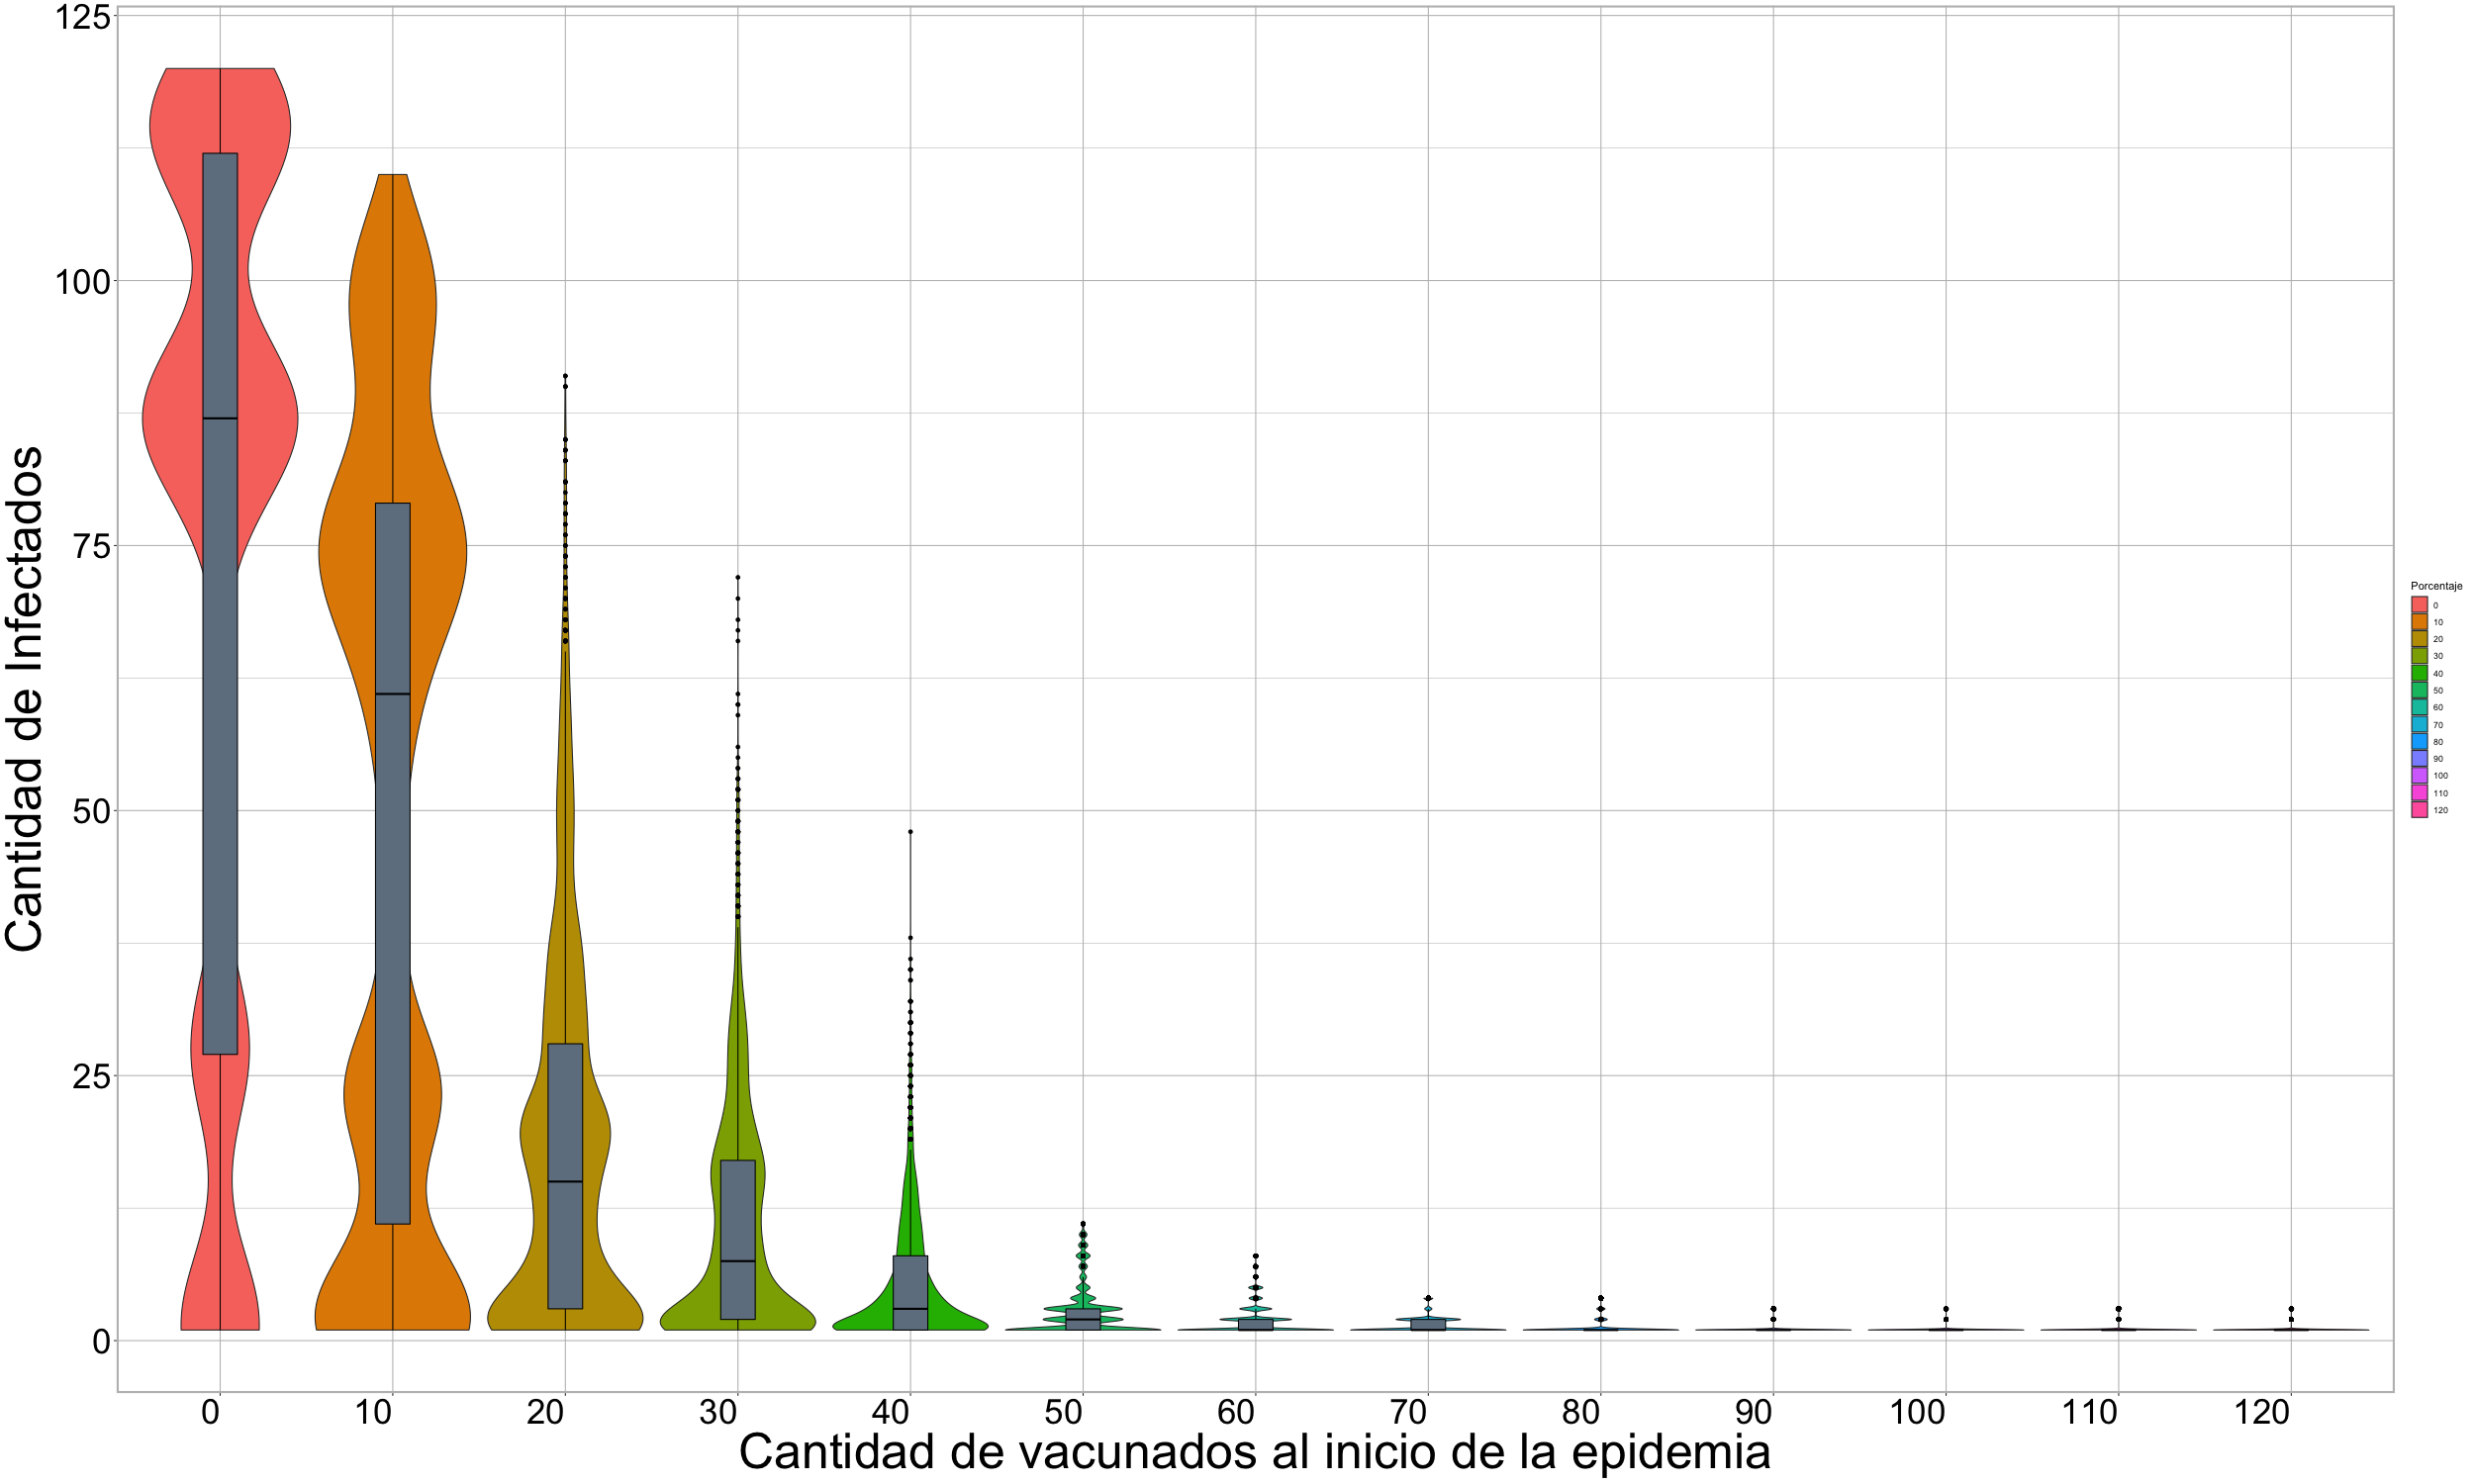
\includegraphics[scale=0.18]{Tesis/img/influential-nodes.png}
    \caption{Vacunando a los nodos influyentes de la red.}
    \label{fig:influential-nodes}
\end{figure}

\begin{figure}
    \centering
    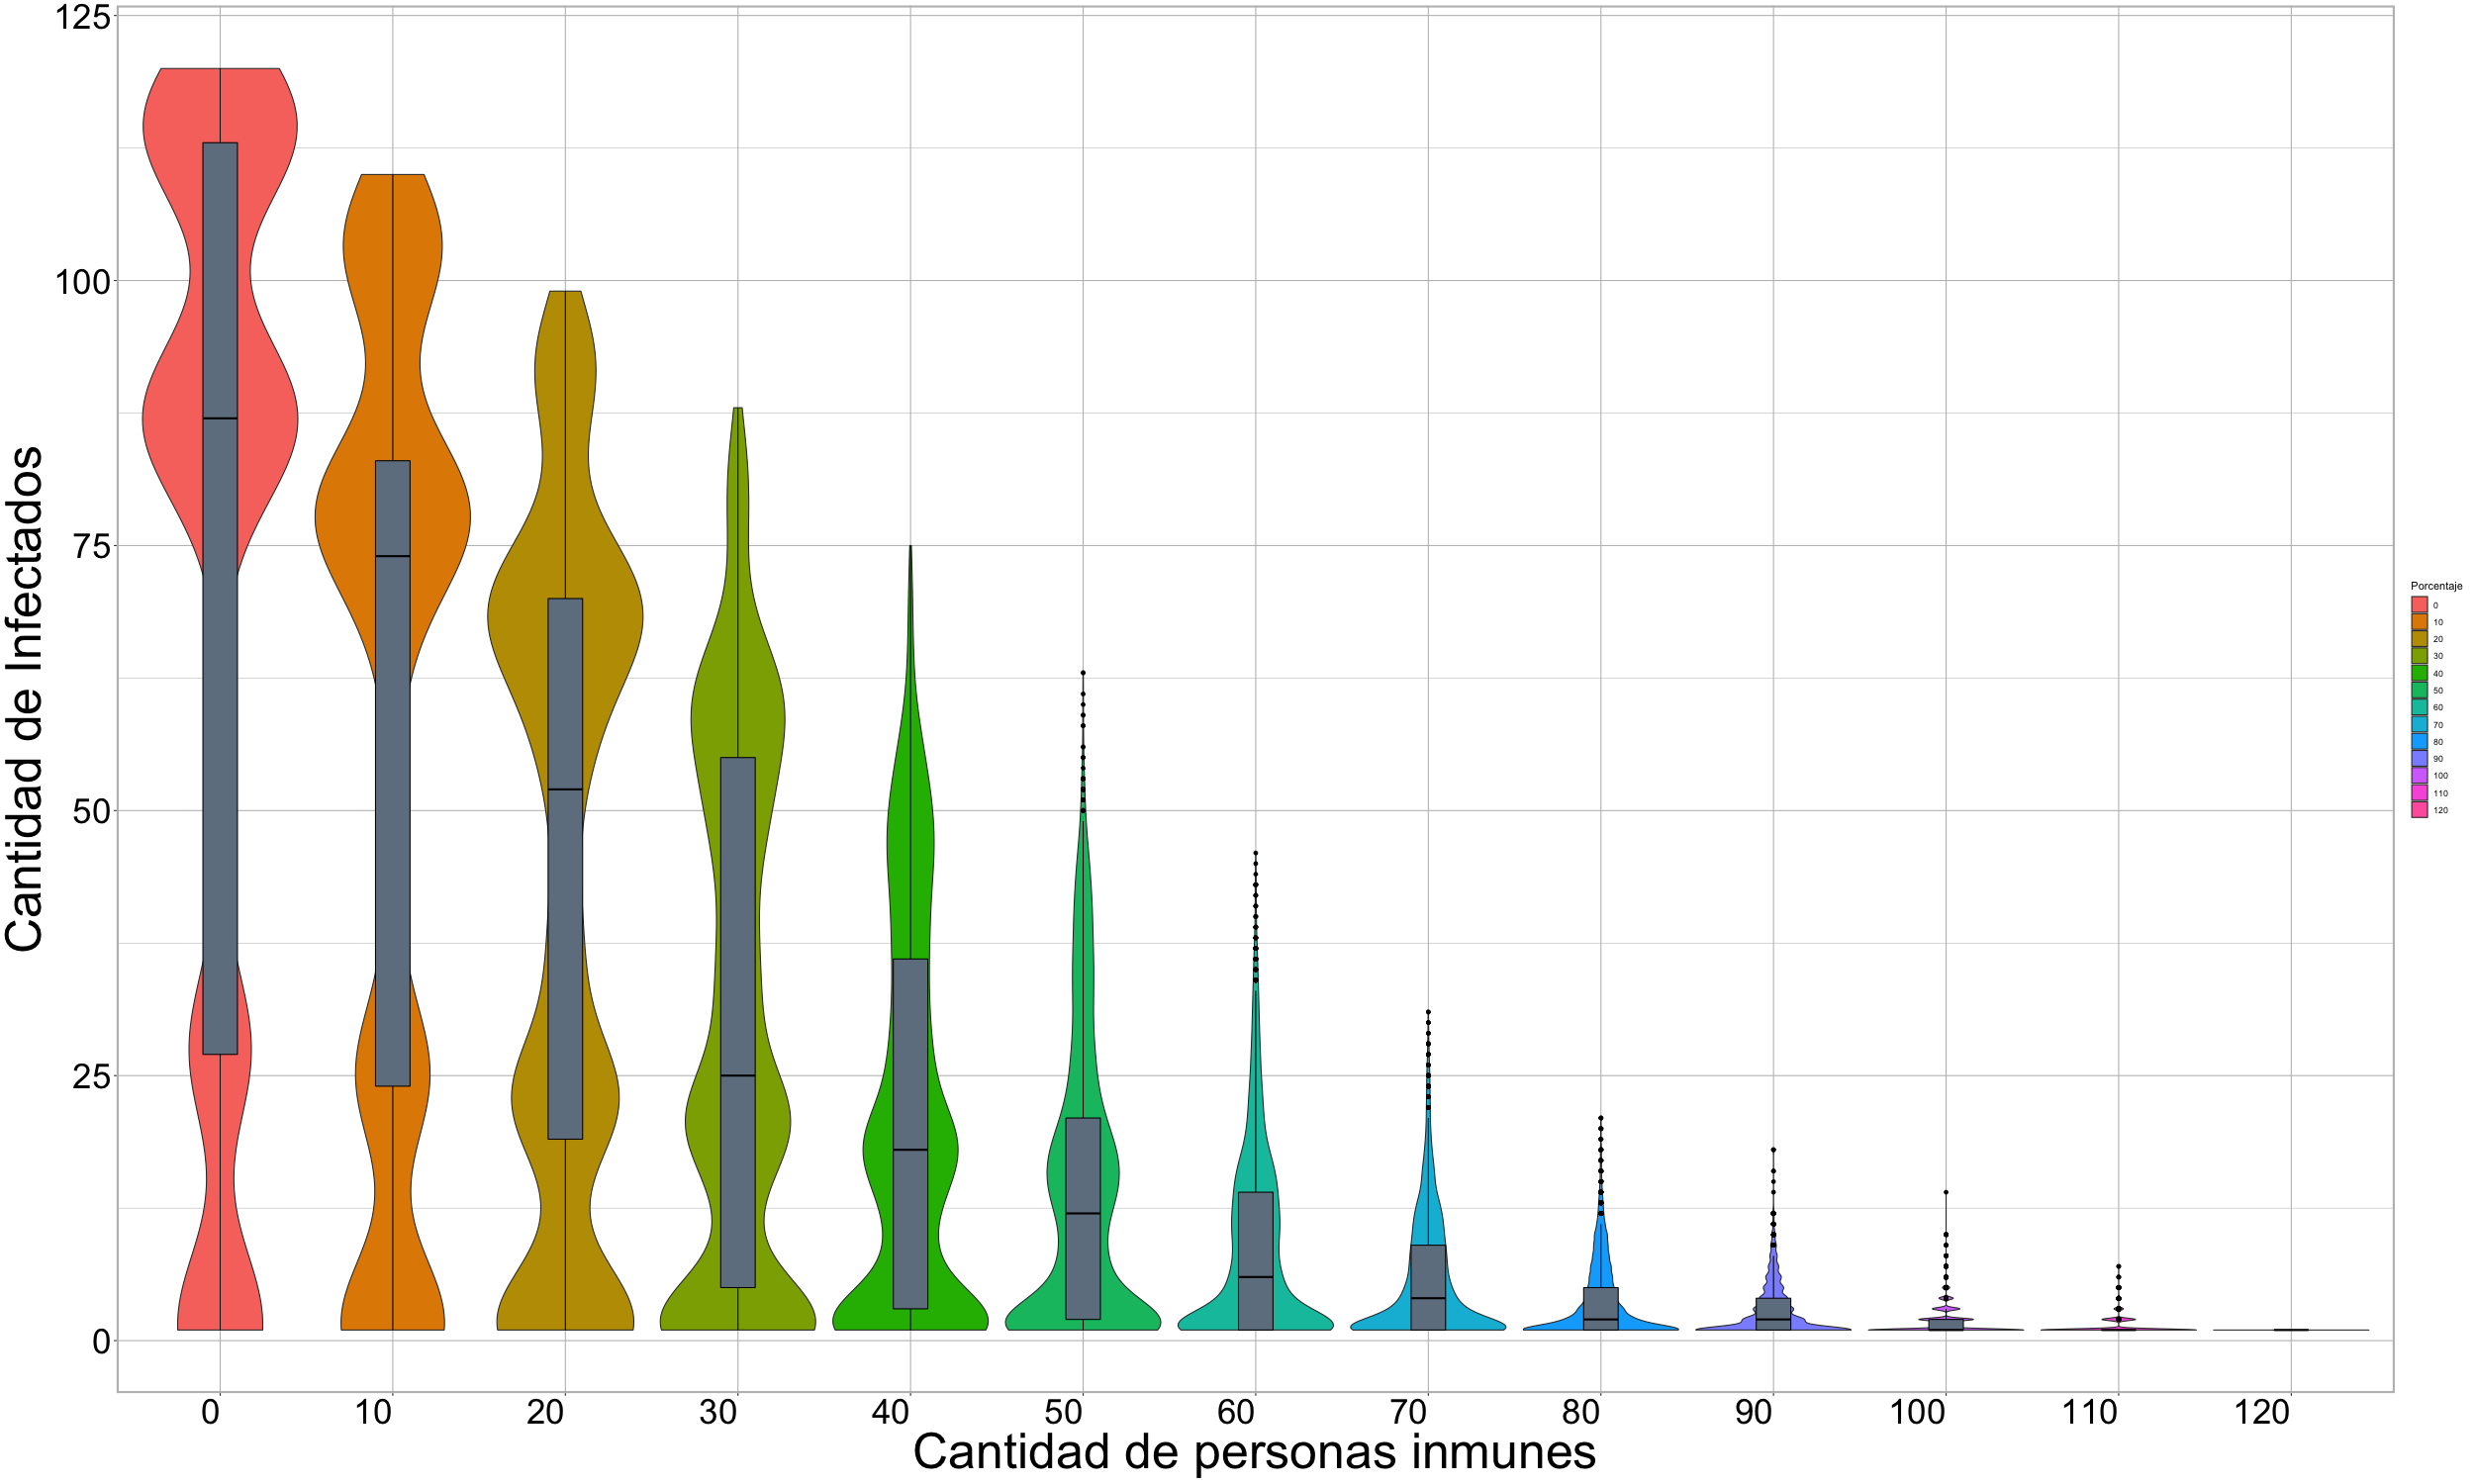
\includegraphics[scale=0.18]{Tesis/img/random.png}
    \caption{Vacunando nodos al azar de la red.}
    \label{fig:random}
\end{figure}

\section{Cubrebocas}



\begin{figure}
    \centering
    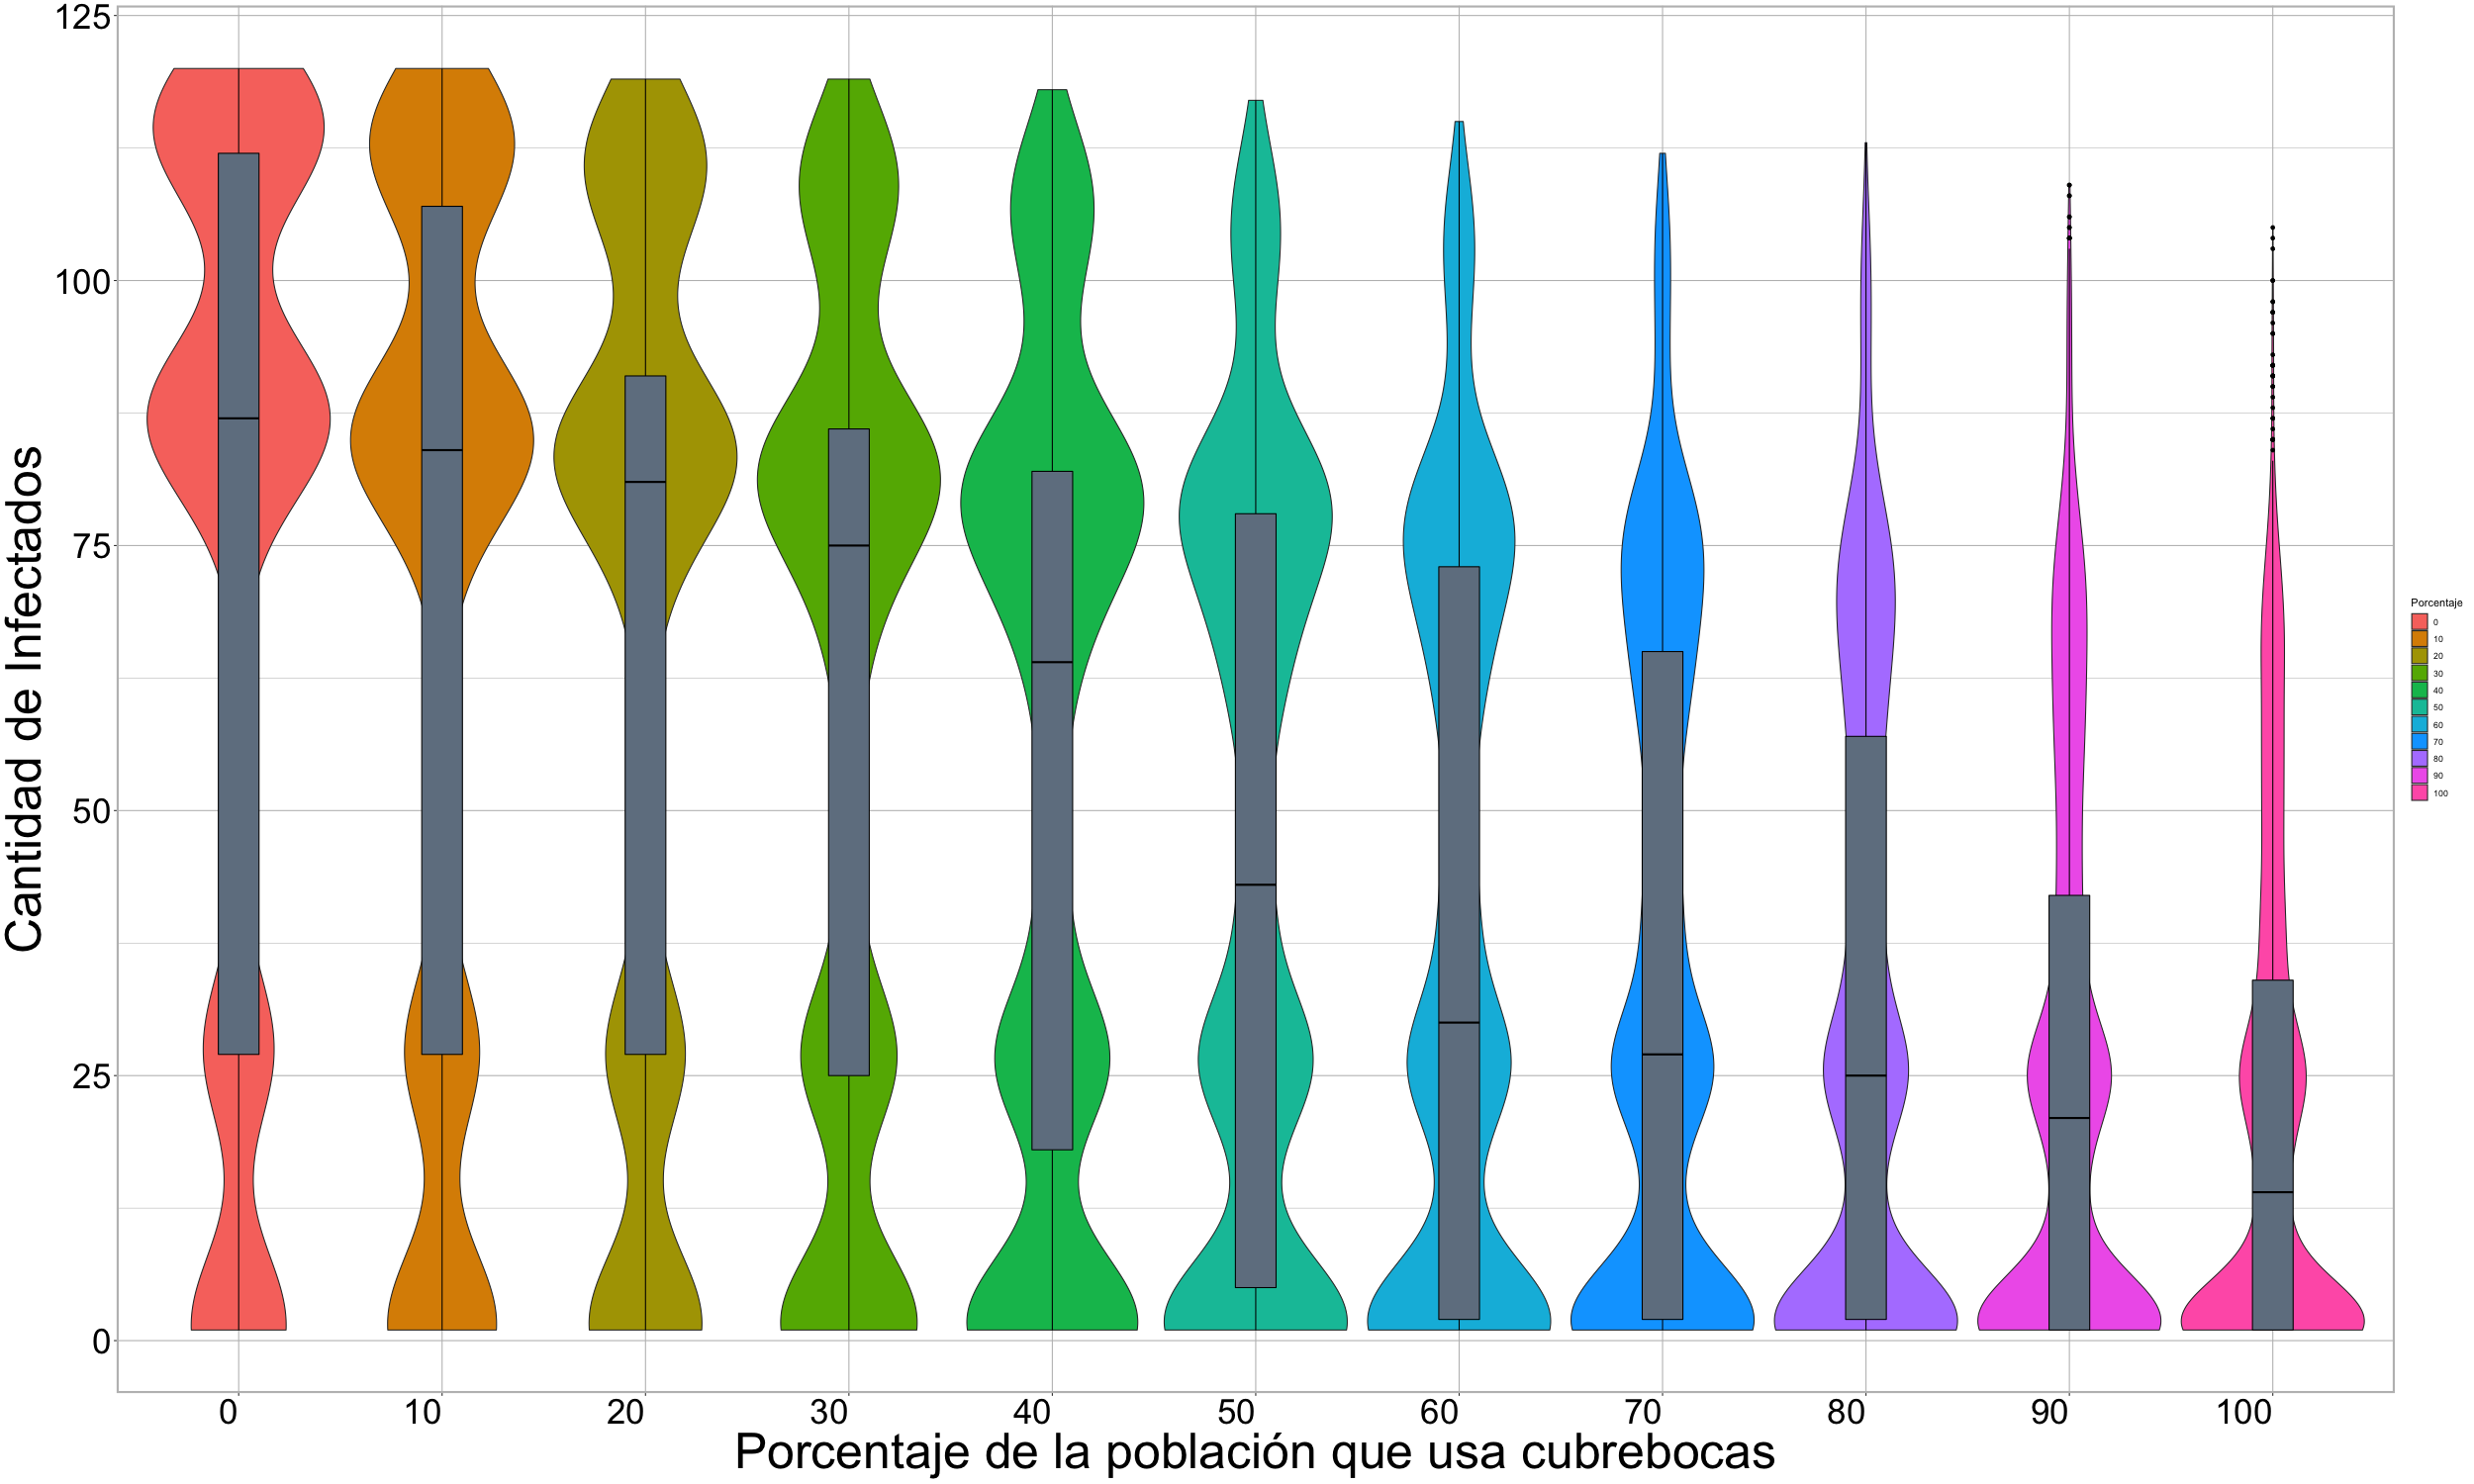
\includegraphics[scale=0.18]{Tesis/img/face-mask.png}
    \caption{Cubrebocas.}
    \label{fig:face-mask}
\end{figure}

\section{Aislamiento}

\begin{figure}
    \centering
    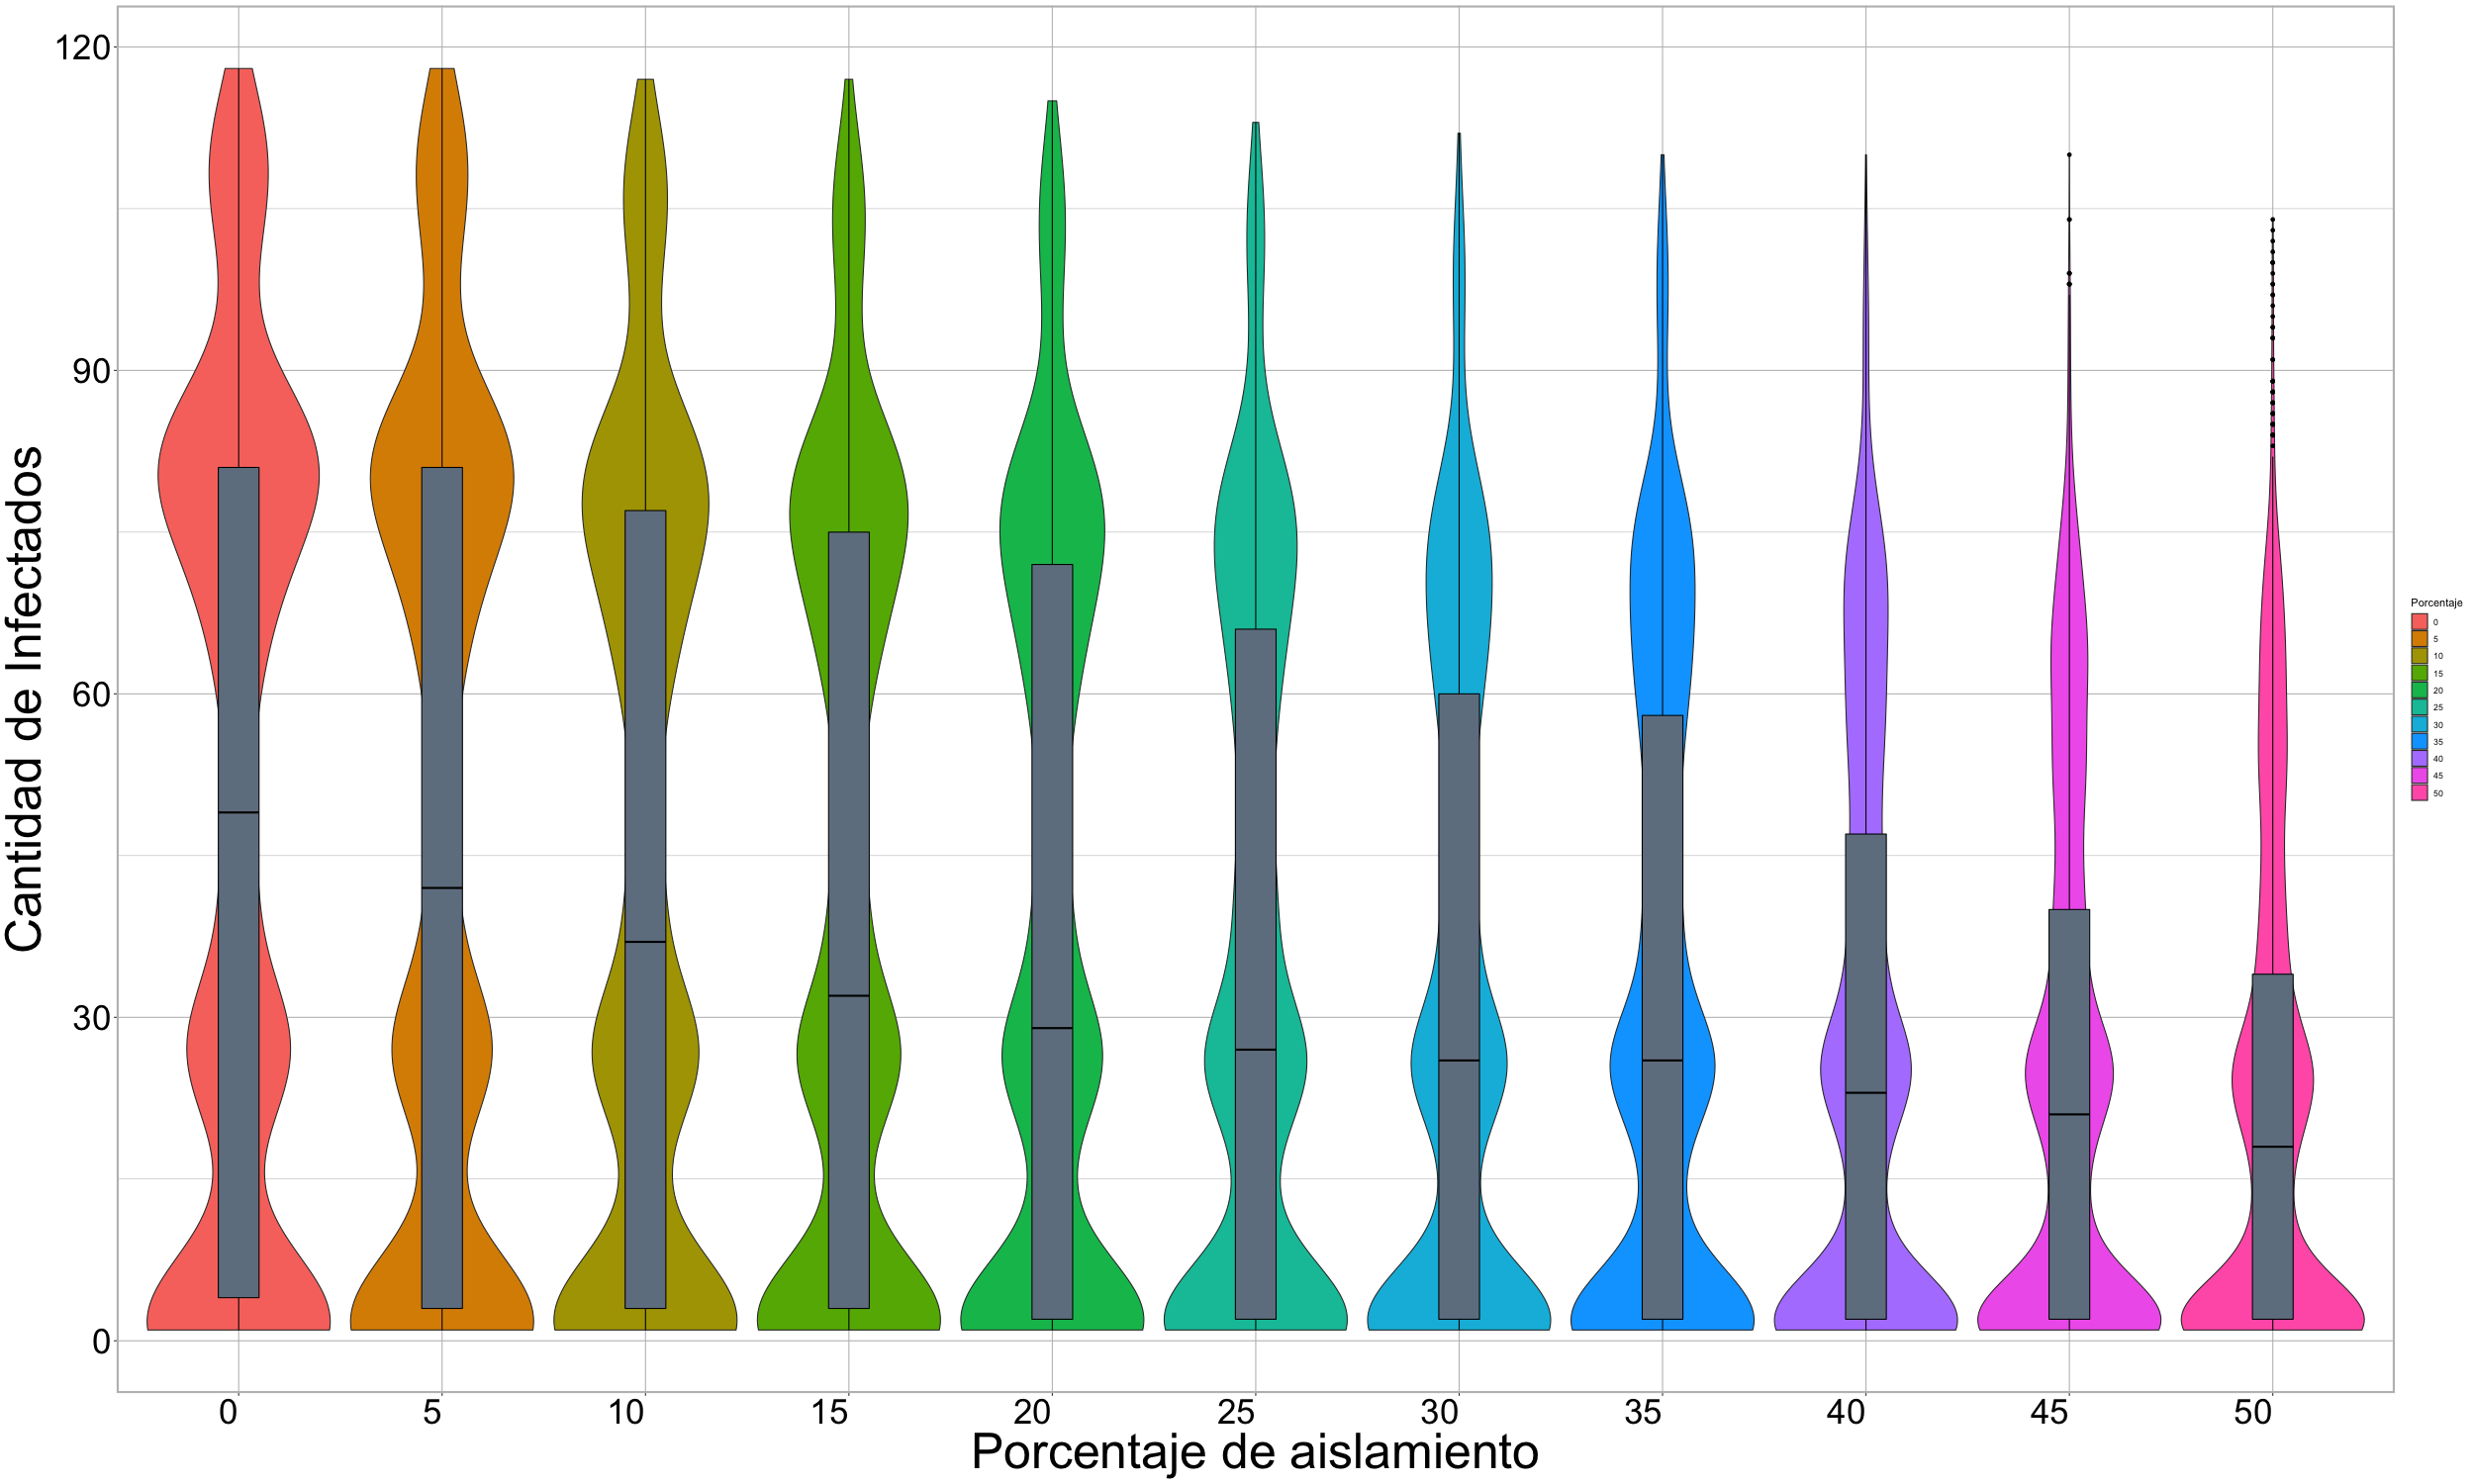
\includegraphics[scale=0.18]{Tesis/img/isolation.png}
    \caption{Aislamiento.}
    \label{fig:isolation}
\end{figure}
\chapter{Conclusiones}\label{ch:conclusions}
\section{Contribuciones}
\section{Trabajo a futuro}

\appendix
%%% Haz un documento para cada apéndice, si es que tienes
%\chapter{Este es un apéndice}

\section{Citas bibliográficas}

En princicpio tienes total libertad de incluir tu bibliografía con el entorno {\tt thebibliography} nativo de \LaTeX{} o mediante la herramienta \textsc{Bib}\TeX. En caso de que optes por esto último (recomendado), puedes usar alguno de los archivos {\tt mighelbib.bst} o {\tt mighelnat.bst} incluidos en el paquete {\tt Tesis-FIME}, pues sus diseños están basados en el estilo bibliográfico estándar del español, además de que armoniza con el estilo de tesis provisto por {\tt fime.cls}.

El estilo bibliográfico {\tt mighelbib} es numérico, es decir cita con un número entre corchetes, por ejemplo una cita \verb+\cite{Dan82}+ genera una etiqueta del tipo [13], mientras que el estilo {\tt mighelnat} es tipo autor-año y requiere que el paquete {\tt natbib} sea cargado (sin opciones) para su correcto funcionamiento, cita con el apellido del autor y el año, por ejemplo una cita \verb+\citet{Dan82}+ genera una etiqueta del tipo Dantzig (1982), mientras que una cita \verb+\citep{Dan82}+ genera una etiqueta del tipo (Dantzig, 1982).

Como muestra del estilo, unas citas: un libro clásico de epidemiología matemática en redes \citep{kiss_mathematics_2017}, o un survey como el de \citet{britton_stochastic_2010}.

\section{Comillas}

El objetivo de esta sección era provocar otra página para que se vea el encabezado. Pero aprovechamos para decir que la clase {\tt fime.cls} carga el paquete {\tt babel} con la opción {\tt spanish}, por lo que cambiará automáticamente los dobles signos $<<$ y $>>$ por << y >>. Estas comillas angulares son las correctas en el idioma español, y son las que se usan en la clase {\tt fime.cls}, por lo que se sugiere sean las usadas en el texto cada que quieras <<entrecomillar>> algo.



\backmatter
\pagestyle{main}


% Aquí va la bibliografía, puedes usar el entorno de LaTeX (thebibliography)
% o la herramienta BibTeX. En caso de que optes por BibTeX, puedes usar
% alguno de los archivos de estilo (mighelbib.bst o mighelnat.bst) incluidos
% en el paquete, cuyos diseños armonizan con el diseño de tesis provisto por
% fime.cls. Para muestra, basta un botón:
%\bibliographystyle{mighelnat}
\bibliographystyle{abbrvnat}
\bibliography{Referencias-tesis}



\label{lastpage}
%Autobiografia

\chapter*{Resumen autobiográfico}
\thispagestyle{empty}

\begin{center}
\autor

Candidato para obtener el grado de\\
\grado\\
\orientacion\bigskip

\uanl\\
\fime\bigskip

Tesis:\\
\textsc{\large\titulo}
\end{center}\bigskip

%Aquí va tu historia
Nací el 29 de octubre de 1994 en la ciudad de Monterrey, Nuevo León; mis padres son Fidel Vázquez Ayala($\dagger$) y María Sanjuana Alcalá Espinosa. En 2016 egresé como Licenciada en Matemáticas en la Facultad de Ciencias Físico-Matemáticas de la Universidad Autónoma de Nuevo León.

%Aquí va tu historia. Recuerda que debe incluir: lugar y fecha de nacimiento, nombre de los padres, escuelas y universidades en las que se graduó después de la preparatoria, títulos o grados obtenidos (no incluir los estudios que se están concluyendo), experiencia profesional y organizaciones profesionales a las que pertenece (no incluir lista de publicaciones).


\end{document}

